%%
%% This is file `sample-sigconf.tex',
%% generated with the docstrip utility.
%%
%% The original source files were:
%%
%% samples.dtx  (with options: `sigconf')
%% 
%% IMPORTANT NOTICE:
%% 
%% For the copyright see the source file.
%% 
%% Any modified versions of this file must be renamed
%% with new filenames distinct from sample-sigconf.tex.
%% 
%% For distribution of the original source see the terms
%% for copying and modification in the file samples.dtx.
%% 
%% This generated file may be distributed as long as the
%% original source files, as listed above, are part of the
%% same distribution. (The sources need not necessarily be
%% in the same archive or directory.)
%%
%%
%% Commands for TeXCount
%TC:macro \cite [option:text,text]
%TC:macro \citep [option:text,text]
%TC:macro \citet [option:text,text]
%TC:envir table 0 1
%TC:envir table* 0 1
%TC:envir tabular [ignore] word
%TC:envir displaymath 0 word
%TC:envir math 0 word
%TC:envir comment 0 0
%%
%%
%% The first command in your LaTeX source must be the \documentclass command.
\documentclass[sigconf]{acmart}
\usepackage{makecell}
\usepackage{multirow}
\usepackage{makecell}  % Add this in your preamble
%%
%% \BibTeX command to typeset BibTeX logo in the docs
\AtBeginDocument{%
  \providecommand\BibTeX{{%
    Bib\TeX}}}
% 調整圖片出現在頁首或頁尾時，與內文之間的距離
\setlength{\textfloatsep}{10pt plus 1.0pt minus 2.0pt}

\setlength{\floatsep}{10pt plus 1.0pt minus 2.0pt}
% 調整圖片出現在兩段文字中間時，上下的距離
\setlength{\intextsep}{10pt plus 1.0pt minus 2.0pt}
%% Rights management information.  This information is sent to you
%% when you complete the rights form.  These commands have SAMPLE
%% values in them; it is your responsibility as an author to replace
%% the commands and values with those provided to you when you
%% complete the rights form.


%%
%% Submission ID.
%% Use this when submitting an article to a sponsored event. You'll
%% receive a unique submission ID from the organizers
%% of the event, and this ID should be used as the parameter to this command.
%%\acmSubmissionID{123-A56-BU3}

%%
%% For managing citations, it is recommended to use bibliography
%% files in BibTeX format.
%%
%% You can then either use BibTeX with the ACM-Reference-Format style,
%% or BibLaTeX with the acmnumeric or acmauthoryear sytles, that include
%% support for advanced citation of software artefact from the
%% biblatex-software package, also separately available on CTAN.
%%
%% Look at the sample-*-biblatex.tex files for templates showcasing
%% the biblatex styles.
%%

%%
%% The majority of ACM publications use numbered citations and
%% references.  The command \citestyle{authoryear} switches to the
%% "author year" style.
%%
%% If you are preparing content for an event
%% sponsored by ACM SIGGRAPH, you must use the "author year" style of
%% citations and references.
%% Uncommenting
%% the next command will enable that style.
%%\citestyle{acmauthoryear}



%%
%% end of the preamble, start of the body of the document source.
\begin{document}

%%
%% The "title" command has an optional parameter,
%% allowing the author to define a "short title" to be used in page headers.
\title{A Spatial Decision Support System for Evaluating POI Addition Suitability via Peer-Relative Context}

% %%
% %% The "author" command and its associated commands are used to define
% %% the authors and their affiliations.
% %% Of note is the shared affiliation of the first two authors, and the
% %% "authornote" and "authornotemark" commands
% %% used to denote shared contribution to the research.



\author{Yen-Tso Chen}
\email{cytso888@gmail.com}
\orcid{0009-0005-8522-7902}
\affiliation{%
  \institution{Department of Computer Science and Engineering, National Chung Hsing University}
  \country{Taiwan}
}



\author{Chien-Yu Yang}
\email{hapqr5678@gmail.com}
\orcid{0009-0003-1910-5494}
\affiliation{%
  \institution{Department of Computer Science and Engineering, National Chung Hsing University}
  \country{Taiwan}
}

\author{Xu-Lin Chen}
\email{charles77778888asd@gmail.com}
\orcid{0009-0001-7137-9826}
\affiliation{%
  \institution{Department of Computer Science and Engineering, National Chung Hsing University}
  \country{Taiwan}
}
\author{An-Syu Li}
\email{yessir0621@gmail.com}
\orcid{0009-0007-9032-1922}
\affiliation{%
  \institution{Department of Computer Science and Engineering, National Chung Hsing University}
  \country{Taiwan}
}



%%

% \author{Sheng-Min Chiu}
% \email{smchiu@cse.nsysu.edu.tw}
% \email{samchiu951010@gmail.com}

% \affiliation{%
%   \institution{Department of Computer Science and Engineering, National Sun Yat-sen University}
%   \country{Taiwan}
% }




\author{Yi-Chung Chen}
\email{chenyich@nchu.edu.tw}
\orcid{0000-0003-0353-7340}
\affiliation{%
  \institution{Department of Computer Science and Engineering, National Chung Hsing University}
  \country{Taiwan}
}


%%
%% By default, the full list of authors will be used in the page
%% headers. Often, this list is too long, and will overlap
%% other information printed in the page headers. This command allows
%% the author to define a more concise list
%% of authors' names for this purpose.

\renewcommand{\shortauthors}{Chen et al.}

%%
%% The abstract is a short summary of the work to be presented in the
%% article.
\begin{abstract}
Within urban geographic information analysis, evaluating the functional composition of spatial grids is critical for understanding regional development. Existing approaches often rely on absolute density estimation or isolated supply-demand metrics, which struggle to determine if a specific region genuinely possesses the structural capacity to support new Point of Interest (POI) additions. To address this limitation, we formulate POI configuration balance as a peer-relative structural assessment. We propose a Spatial Decision Support System that evaluates the suitability of POI additions by learning the expected functional composition from surrounding urban contexts. Our framework leverages TF-IDF preprocessing to highlight functionally discriminative POIs, constructs a k-nearest-neighbor graph to capture functional peer relationships, and employs a Denoising Autoencoder optimized jointly with a Fuzzy Simplicial Set Cross-Entropy (FSCE) loss to preserve high-dimensional topology in a low-dimensional latent space. Experiments on real-world check-in data show that the learned representation retains the POI composition while preserving peer relationships, and case studies illustrate how the system can provide urban planners with an interpretable, data-driven tool to explore facility expansion scenarios.
\end{abstract}
%%
%% The code below is generated by the tool at http://dl.acm.org/ccs.cfm.
%% Please copy and paste the code instead of the example below.
%%
% \begin{CCSXML}
% <ccs2012>
%  <concept>
%   <concept_id>10010520.10010553.10010562</concept_id>
%   <concept_desc>Computer systems organization~Embedded systems</concept_desc>
%   <concept_significance>500</concept_significance>
%  </concept>
%  <concept>
%   <concept_id>10010520.10010575.10010755</concept_id>
%   <concept_desc>Computer systems organization~Redundancy</concept_desc>
%   <concept_significance>300</concept_significance>
%  </concept>
%  <concept>
%   <concept_id>10010520.10010553.10010554</concept_id>
%   <concept_desc>Computer systems organization~Robotics</concept_desc>
%   <concept_significance>100</concept_significance>
%  </concept>
%  <concept>
%   <concept_id>10003033.10003083.10003095</concept_id>
%   <concept_desc>Networks~Network reliability</concept_desc>
%   <concept_significance>100</concept_significance>
%  </concept>
% </ccs2012>
% \end{CCSXML}

% \ccsdesc[500]{Computer systems organization~Embedded systems}
% \ccsdesc[300]{Computer systems organization~Redundancy}
% \ccsdesc{Computer systems organization~Robotics}
% \ccsdesc[100]{Networks~Network reliability}

%%
%% Keywords. The author(s) should pick words that accurately describe
%% the work being presented. Separate the keywords with commas.
% \copyrightyear{2025}
% \acmYear{2025}
% \setcopyright{cc}
% \setcctype{by}
% \acmConference[AICCC 2025]{2025 8th Artificial Intelligence and Cloud Computing Conference}{December 20--22, 2025}{Tokyo, Japan}
% \acmBooktitle{2025 8th Artificial Intelligence and Cloud Computing Conference (AICCC 2025), December 20--22, 2025, Tokyo, Japan}
% \acmPrice{}
% \acmDOI{10.1145/3789982.3790066}
% \acmISBN{979-8-4007-1889-2/2025/12}

\begin{CCSXML}
<ccs2012>
   <concept>
       <concept_id>10002951.10003227.10003236</concept_id>
       <concept_desc>Information systems~Spatial-temporal systems</concept_desc>
       <concept_significance>500</concept_significance>
       </concept>
 </ccs2012>
\end{CCSXML}
\ccsdesc[500]{Information systems~Spatial-temporal systems}
% \ccsdesc[500]{Information systems~Geographic information systems}
\keywords{Point of Interest, Spatial Decision Support System, Structural Balance, Representation Learning, Locational Optimization}
% %% A "teaser" image appears between the author and affiliation
% %% information and the body of the document, and typically spans the
% %% page.

\maketitle
%%
%% This command processes the author and affiliation and title
%% information and builds the first part of the formatted document.
\section{Introduction}
Within urban geographic information analysis, evaluating the functional composition of spatial grids is a pivotal task for understanding how Points of Interest (POIs) shape regional development. A central but often overlooked property of urban POIs is that they rarely function in isolation: different facility categories interact in complementary ways, where one type of POI effectively expands what the surrounding area is able to support. For instance, transit stops absorb and redistribute the foot traffic generated by a dense cluster of dining options, allowing the same area to sustain a higher concentration of restaurants without becoming overloaded. We refer to this complementary relationship as a region's \textit{structural capacity}, defined as the extent to which the existing functional composition can carry a given facility. When this capacity is adequately matched, as shown in the left panel of Figure \ref{fig:poi_saturation_example}, a dense cluster of amenities remains a healthy, well-supported configuration. When it is not, as in the right panel, the same density becomes an over-concentrated configuration that exceeds what the local context can carry. This distinction reveals that the suitability of a POI addition is not determined by its absolute count, but by whether it remains proportionate to the structural capacity established by its surrounding functions, a property we refer to as a region's structural balance. Consequently, the primary problem addressed in this study is how to evaluate whether a hypothetical POI addition remains structurally balanced relative to the functional composition observed in comparable urban regions. In this work, we operationalize structural balance through peer typicality: we assume that a composition close to those of functionally comparable regions is structurally balanced. We note that this is a working assumption rather than a planning judgment, since specialized districts (e.g., airports) may legitimately deviate from their peers.

\begin{figure}[htbp]
    \centering
    % Ensure the image file is in the same directory as your .tex file
    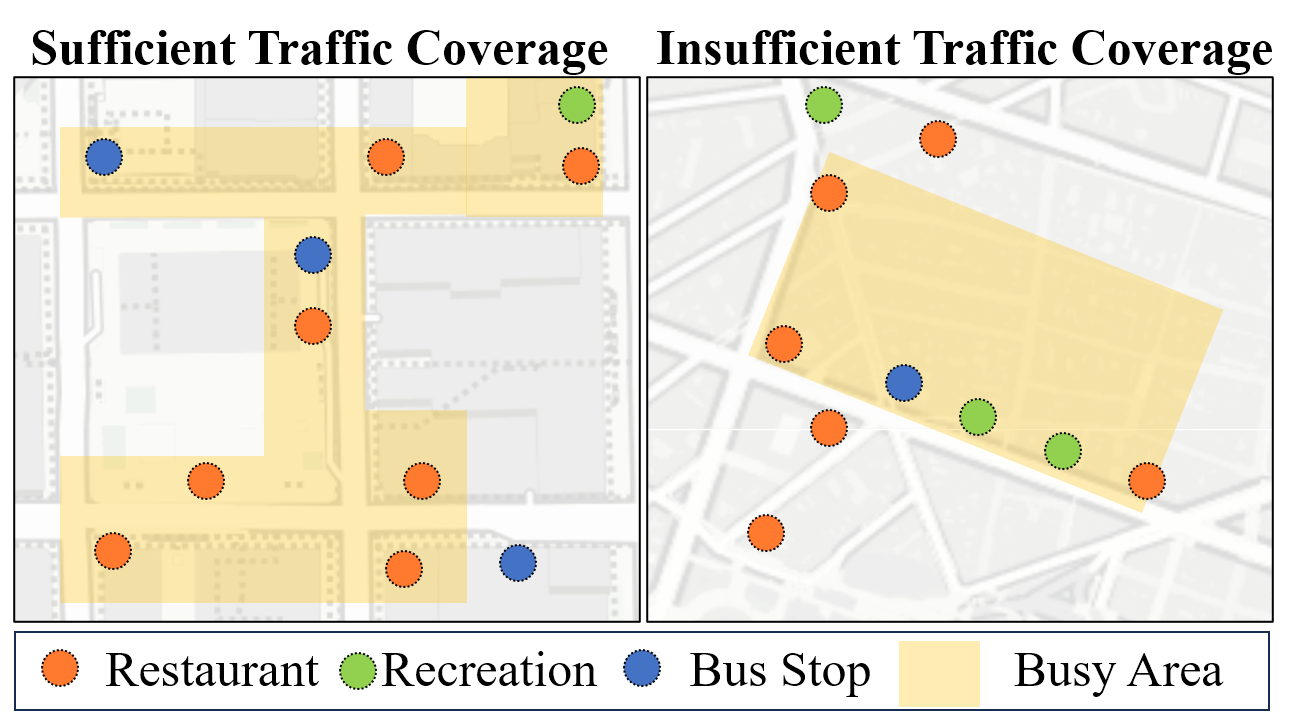
\includegraphics[width=.9\linewidth]{figure/poi_saturation_example.png}
    \caption{Comparison of POI distributions using peer context: a reasonable co-cluster aggregation near a transit hub (left) versus a structural imbalance in a residential alley (right).}
    \label{fig:poi_saturation_example}
\end{figure}

Despite the practical importance of this problem, urban POI structural balance has not been extensively studied as a problem of learning the expected functional composition of a spatial area from its surrounding context. Existing approaches provide several related perspectives, including supply and demand analysis, POI-based site selection, and urban functional-zone identification. For example, Gao et al.~\cite{Gao03072019} incorporated population and facility information to identify potential over-supply zones; however, their method remains focused on facility-specific supply measures and does not explicitly model the functional relationships among heterogeneous POI categories. To address functional linkages, Hidalgo et al.~\cite{hidalgo2020amenity} modeled neighborhood amenity mixes from observed co-location relationships and identified over- and under-supplied amenities. From a demand-oriented perspective, Niu et al.~\cite{niu2016exploiting} relied on human mobility patterns to estimate gas-station demand. Adding to this, Chen et al.~\cite{chen2025research} evaluated the spatial supply-demand balance of community public service facilities and its driving mechanisms, yet their analysis has not addressed the structural connections across multi-category POIs. In the domain of POI-based site selection, Han et al.~\cite{HAN2022416} emphasized the importance of measuring location similarity, demonstrating through an international restaurant chain case that a candidate site structurally analogous to an existing profitable store will likely yield comparable sales. However, this approach remains focused on brand-specific retail-site recommendation rather than evaluating the complete multi-category composition of a region. Along similar lines, studies by Zhao et al.~\cite{zhao2025site} on retail stores, Mazhi et al.~\cite{inproceedings} on shop site selection, and Liu et al.~\cite{7373406} on bike-sharing systems commonly characterize competition through local POI density or spatial proximity. Yet such density-based criteria cannot distinguish a high-density area that is structurally supported by complementary functions from one that is genuinely imbalanced. Similarly, regarding urban functional-zone identification, Guo et al.~\cite{guo2023shape} utilized a shape-and-size-free CNN to map irregular functional zones from satellite imagery and POI data. However, their approach focuses on image features and discrete classification, without explicitly modeling the functional composition similarity among different regions. Other works share this descriptive focus; Miao et al.~\cite{miao2021analyzing} utilized clustering, Xu et al.~\cite{xu2023identification} applied graph-based learning, and Gao et al.~\cite{gao2017extracting} employed latent topic models to characterize urban functional composition. Ultimately, these approaches primarily aim to classify or describe existing urban functions rather than determine whether the observed composition of a specific area is structurally disproportionate relative to comparable areas. More fundamentally, existing approaches do not simultaneously provide a data-driven balance criterion, a multi-category representation of the complete POI composition, and a peer-based reference that captures the functional context in which a POI cluster occurs.

To address this under-explored problem, we explicitly formulate POI-addition suitability as a peer-relative structural balance problem and develop a dedicated framework specifically for this setting, rather than treating facility expansion as a conventional density, demand, or outcome-prediction problem. The key idea is to first represent each spatial patch by its complete multi-category POI composition and then identify functionally similar patches as peers, allowing the expected configuration of a target area to be inferred from structurally comparable urban contexts. To obtain a discriminative representation, we apply Term Frequency-Inverse Document Frequency (TF-IDF) to the category counts. This mathematical transformation suppresses highly prevalent and weakly discriminative categories while emphasizing categories that better distinguish local functional characteristics. We then construct a $k$-nearest-neighbor graph using cosine similarity in the TF-IDF space and employ fuzzy simplicial set cross-entropy (FSCE) to preserve the resulting high-dimensional functional relationships in a low-dimensional latent space. In this way, the representation retains not only the categorical data required to reconstruct the original POI composition but also the topology of functional similarity among urban patches. Combined with a denoising objective, the resulting latent functional space provides a robust geometric basis for peer comparison. This mechanism enables the proposed framework to distinguish a contextually supported POI aggregation from a structurally imbalanced concentration.  

The proposed framework operationalizes this locational assessment logic through a continuous four-stage computational pipeline. In the initial phase, raw spatial coordinates of POIs are aggregated into regular grid patches and converted into discrete category-count vectors. The system then applies a TF-IDF transformation to these vectors and calculates cosine similarity to construct a functional $k$-nearest-neighbor graph. During the third stage, a denoising autoencoder projects the discrete data into a continuous latent representation by jointly optimizing a Poisson reconstruction loss and a FSCE objective, which mathematically encodes the graph topology. In the final stage, the learned latent space is queried during online inference to establish peer-based contextual comparisons. These comparisons allow the system to quantitatively assess the structural balance of existing spatial distributions and evaluate trajectory shifts caused by the hypothetical introduction of additional facilities. 

\section{Related Work}

Research on POI-based urban analytics has been extensively studied over the years. Existing studies can be broadly grouped according to the role they play in this problem: representing the functional composition of urban regions, learning spatial and relational dependencies among urban regions, and supporting location-related decision making. Accordingly, we review prior work from three perspectives: POI-based urban representation, spatial and relational urban representation learning, and data-driven retail location evaluation.

\subsection{POI-Based Urban Representation}

Research on POI-based urban representation has focused on transforming POI distributions and contextual relationships into representations of urban functions. Luo et al.~\cite{luo2023urban} developed an urban functional-zone classification approach based on kernel-density features of reclassified POI functional types. Yan et al.~\cite{yan2017place2vec} introduced Place2Vec to learn place-type embeddings from augmented spatial contexts incorporating geographic distance, activity, and type uniqueness. Yang et al.~\cite{yang2023classifying} organized POIs as graphs and employed DeepWalk to learn embeddings that capture spatial relationships among geographic elements, which were subsequently aggregated for urban functional-zone representation. Together, these studies establish POI distributions, contextual information, and structural relationships as informative signals for characterizing regional urban functions.

\subsection{Spatial and Relational Urban Representation Learning}

Another line of research has focused on incorporating spatial and relational dependencies into learned urban representations. Xu et al.~\cite{xu2023spatial} proposed a spatial and adversarial representation-learning framework that combines CNN-based spatial encoding with autoencoder reconstruction and adversarial learning to capture POI spatial and categorical information. ReCP jointly employed feature reconstruction, intra-view contrastive learning, and cross-view prediction to learn consistent region representations from POI and human-mobility views~\cite{li2024urban}. HGI modeled POI- and region-level interactions through graph convolution and hierarchical mutual-information maximization~\cite{huang2023learning}. Fan et al.~\cite{fan2024neural} further used graph neural networks to learn urban-area embeddings from heterogeneous urban features and mobility interactions, and employed UMAP to visualize the resulting spatial structures. Collectively, these studies demonstrate how spatial configuration, graph relations, cross-view consistency, and mobility interactions can contribute to structured urban representations.

\subsection{Data-Driven Retail Location}

Data-driven retail research has further translated urban and spatial information into location-related decision support. Ouyang et al.~\cite{ouyang2020site} proposed a spatial competition index together with a double-channel convolutional neural network to estimate regional market demand and recommend retail sites with high market potential. Lan et al.~\cite{lan2022site} constructed a geospatial graph convolutional network that integrates local land-use information with spatial and public-transport connectivity to predict store-site attractiveness. D'Silva et al.~\cite{dsilva2018role} identified discriminative venue-specific, neighborhood, and mobility features and used them to predict retail business survival. These studies establish that spatial competition, neighborhood context, connectivity, and mobility information can be operationalized to support data-driven retail location decisions.

\subsection{Positioning of This Study}

These three lines of research provide complementary foundations for the problem considered in this study. POI-based representation studies demonstrate how regional functions can be encoded from POI composition and contextual relationships; spatial and relational representation methods provide mechanisms for incorporating structured dependencies into urban embeddings; and data-driven retail studies show how urban information can be translated into location-related evaluations. Our problem, however, requires these capabilities to operate within a single intervention-oriented framework. Specifically, the evaluation must identify functionally comparable regions, preserve these peer relationships in the latent space used for comparison, and provide a parameterized mapping through which a modified POI composition can be re-encoded to quantify its change relative to the same functional context. The reviewed studies primarily address these components for representation, relational learning, or outcome prediction, rather than integrating them for peer-relative evaluation of hypothetical POI additions.

\section{Method}
\label{sec:method}

According to Figure~\ref{fig:method}, this section consists of the Offline Process for model training and the Online Process for user interaction and evaluation, strictly following the data flow illustrated in the system architecture.
\begin{figure}[htbp]
    \centering
    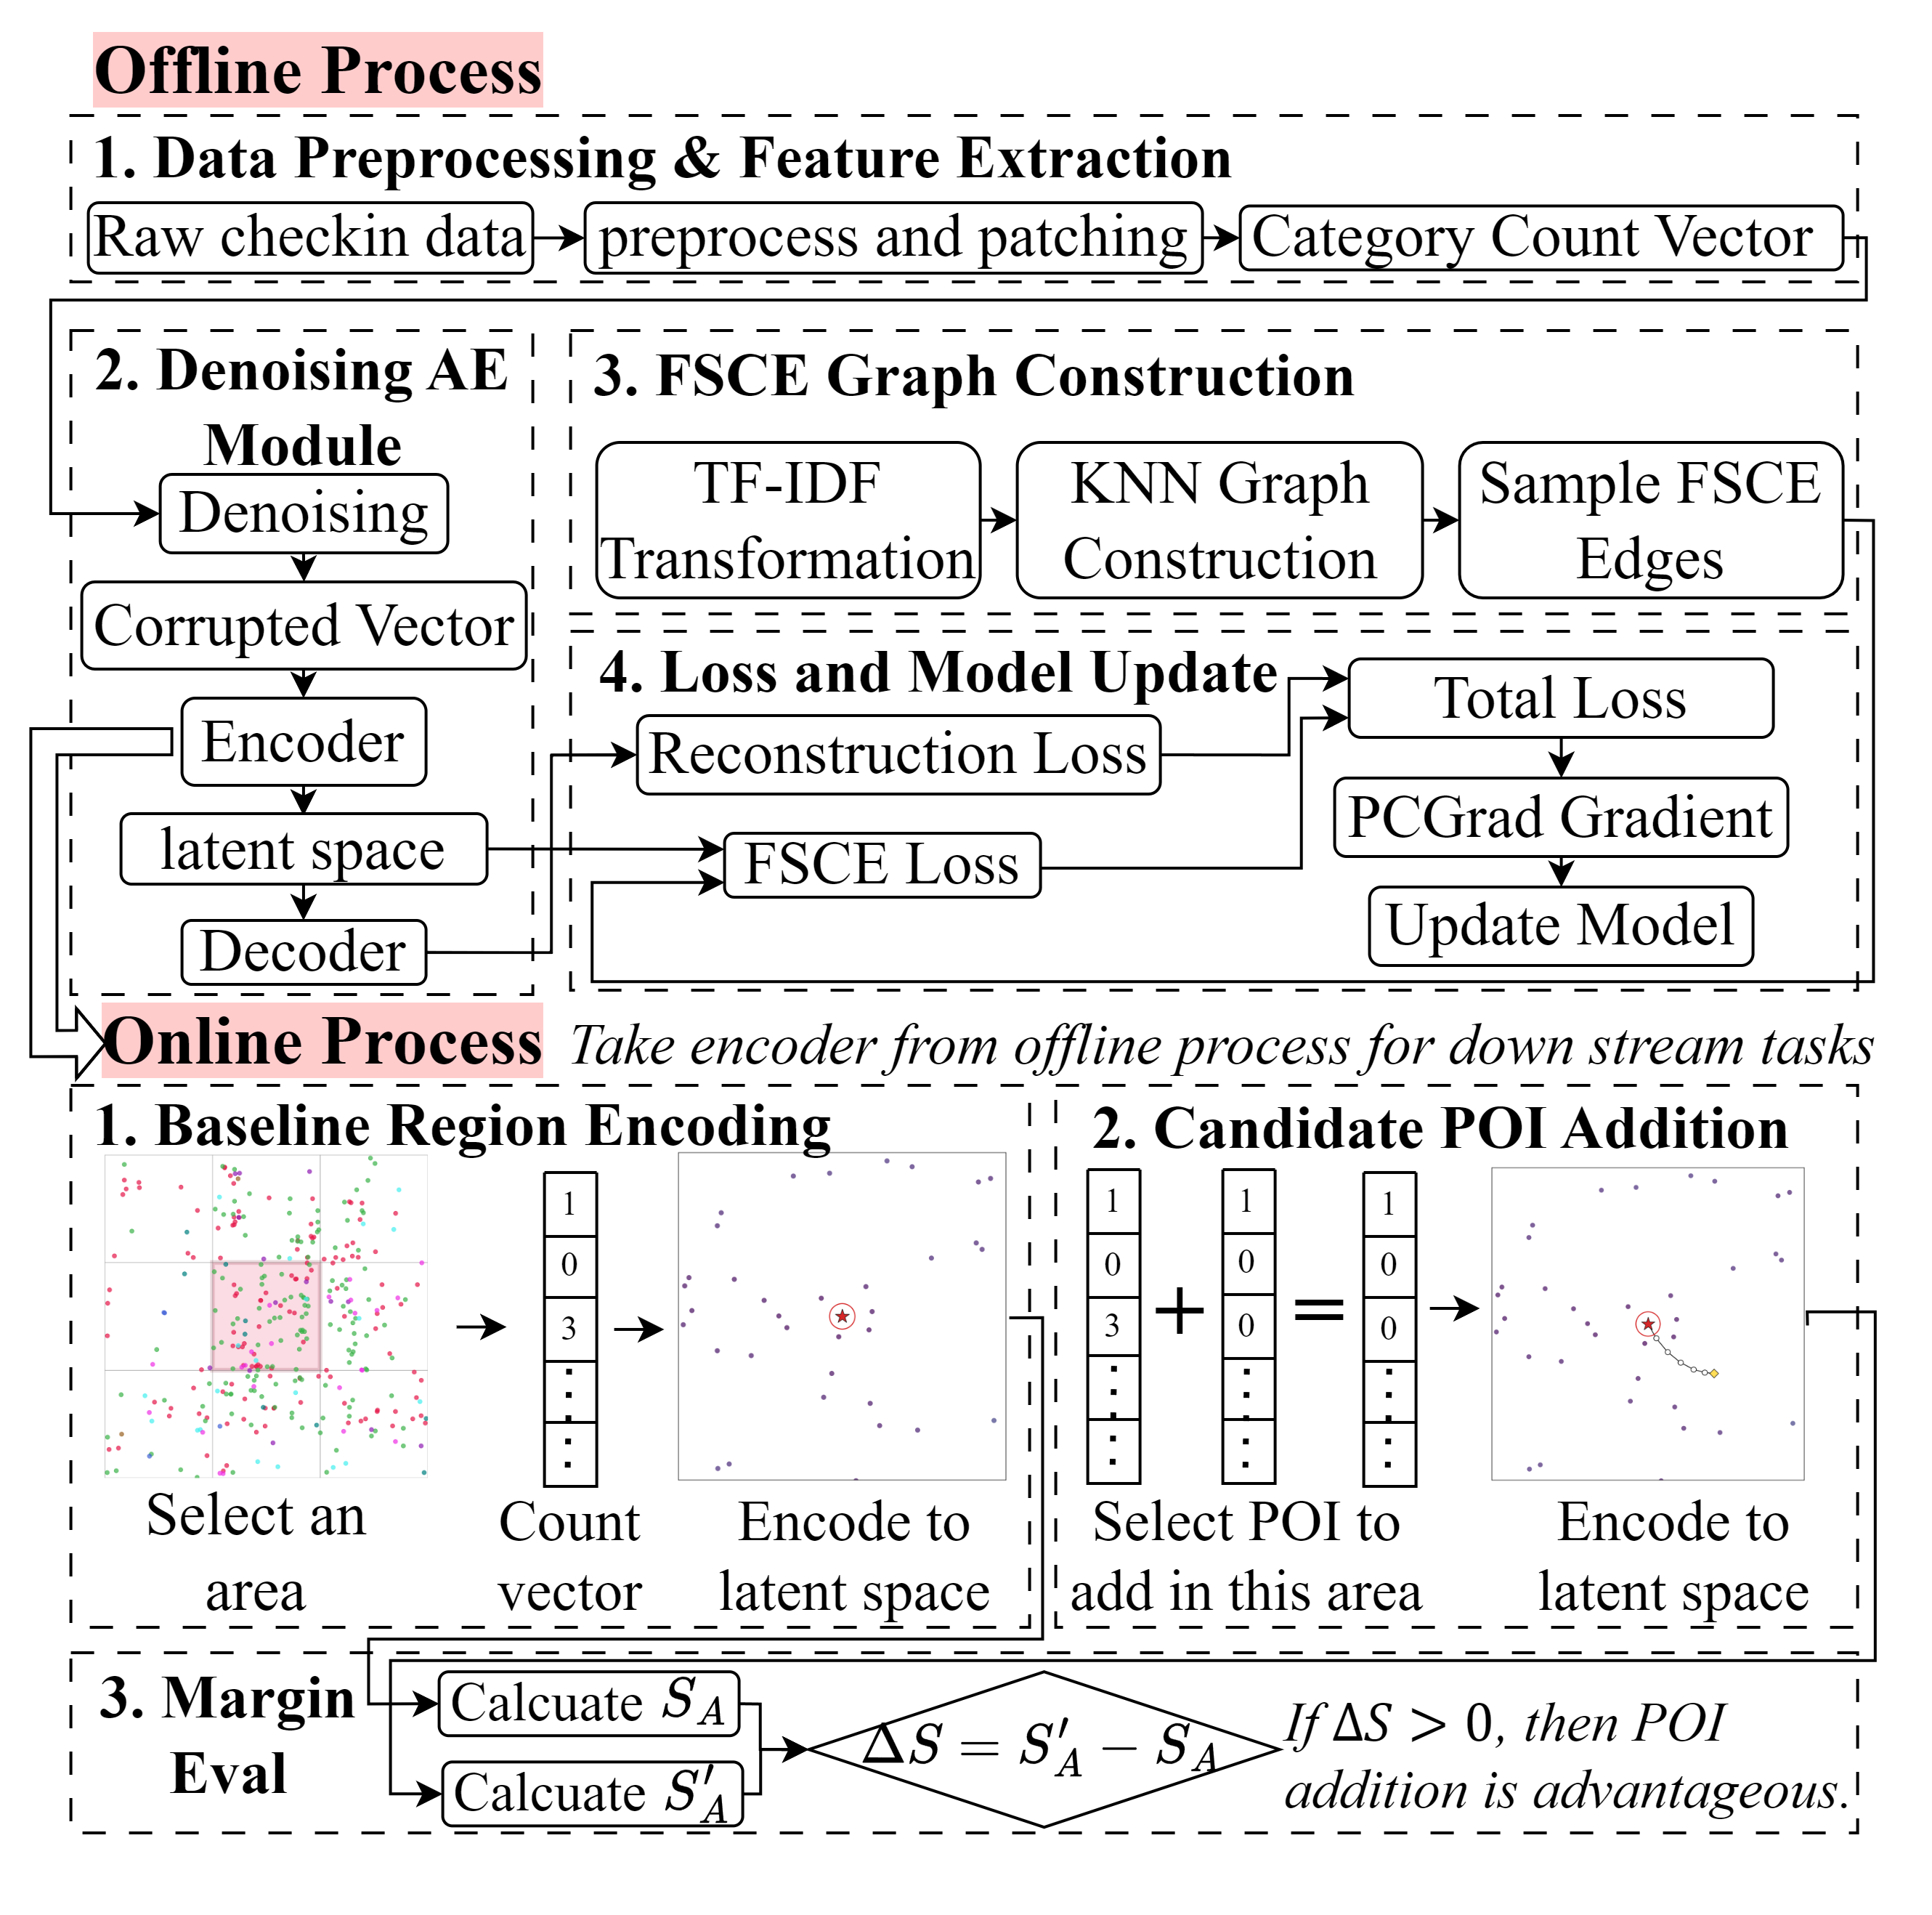
\includegraphics[width=\linewidth]{figure/method}
    \caption{System architecture illustrating the data flow of the Offline Process for model training and the Online Process for user interaction and evaluation.}
    \label{fig:method}
\end{figure}
\subsection{Offline Process}
The offline process encompasses the data preparation, functional graph construction, and joint training of a denoising autoencoder. This stage is designed to learn a robust latent representation of the spatial configurations from the historical dataset, which serves as the foundation for downstream peer comparisons.

\paragraph{Raw Check-in Data, Preprocessing, and Patching}
The pipeline begins with raw check-in data collected from Foursquare Tokyo. Each record consists of the POI coordinates and its category, utilizing the top-level categories from the official Foursquare hierarchy ($C=10$). For spatial consistency, the raw WGS84 coordinates are projected into the Japanese Rectangular Coordinate System Zone 9 (EPSG:6677) in meters. The projected plane is partitioned into a regular grid with a side length of $s$. To ensure statistical significance and filter out overly sparse areas, only grids containing a total POI count $|N_i| \ge n_{\min}$ are retained as valid patches for further processing.

\paragraph{Category Count Vector}
For each valid patch, the occurrences of each POI category are aggregated to form a Category Count Vector $x_i$. The count for each category $c$ is defined as:
\begin{equation}
x_{i,c}=\sum_{q\in N_i}\mathbb{1}[\text{cat}(q)=c],\quad c=1,\dots,C
\end{equation}
From this vector, the offline process splits into two parallel representation branches: Graph Construction and Autoencoder Training.

\paragraph{KNN Graph Construction \& Sample FSCE Edges}
To capture the functional context and peer relationships, the entire matrix of count vectors $X\in\mathbb{Z}^{N\times C}$ undergoes a TF-IDF transformation (with L2 normalization and smoothed IDF). This transformation is a direct methodological response to the extreme categorical imbalance observed in the spatial dataset. In real-world urban environments, ubiquitous categories like dining and retail often overshadow critical but less frequent infrastructural features. By applying TF-IDF, the system mathematically suppresses these globally dominant, weakly discriminative categories while emphasizing the specific functions that truly distinguish local spatial characteristics. The formulas are defined as follows:
\begin{equation}
\text{idf}_c=\ln\frac{1+N}{1+\text{df}_c}+1,\qquad \tilde x_{i,c}=\frac{x_{i,c}\cdot\text{idf}_c}{\lVert x_{i,\cdot}\odot\text{idf}\rVert_2}
\end{equation}
In this TF-IDF space, a K-Nearest-Neighbor (KNN) Graph Construction is performed using cosine distance to find the $k=10$ nearest peers. Following the UMAP algorithm, a fuzzy simplicial set is constructed to generate the edge set $(i,j)$ and corresponding edge weights $w_{ij}\in[0,1]$, while deriving the kernel parameters $(a,b)$. This graph is exclusively built on the training set. During training, we sample FSCE Edges by randomly drawing a specific batch of positive edges $(i,j,w_{ij})$ and uniformly sampling an equal number of negative edges (randomly paired with weight 0) for contrastive learning. 

\paragraph{Denoising \& Corrupted Vector}
In parallel, the original category count vector is subjected to a Denoising process via a thinning destruction mechanism. Real-world spatial point data is inherently noisy and susceptible to uneven sampling bias. To prevent the model from merely memorizing absolute POI counts and to force it to learn the underlying structural balance, each count unit is independently retained with a probability of $\text{keep}=1-p$. The resulting Corrupted Vector is then unbiasedly scaled:
\begin{equation}
\hat x_{i,c}=\frac{1}{1-p}\sum_{u=1}^{x_{i,c}} \text{Bernoulli}(1-p)_u,\qquad \mathbb{E}[\hat x_{i,c}]=x_{i,c}
\end{equation}

\paragraph{Encoder, Latent Space, and Decoder}
The Corrupted Vector $\hat x_i$ is fed into the Encoder $f_\theta:\mathbb{R}^C\to\mathbb{R}^d$, which consists of 4 layers of Linear $\rightarrow$ LayerNorm $\rightarrow$ GELU (with hidden dimension $h$) and a final linear projection to map the data into a low-dimensional Latent Space $d$:
\begin{equation}
z_i=f_\theta(\hat x_i)
\end{equation}
The Decoder $g_\theta:\mathbb{R}^d\to\mathbb{R}^C$ applies a symmetric architecture to reconstruct the original vector from the latent space by outputting the log-rate parameters:
\begin{equation}
\log\hat\lambda_i=g_\theta(z_i)
\end{equation}
The network is optimized using a joint loss function. The reconstruction uses a Poisson negative log-likelihood loss $\mathcal{L}_{\text{recon}}$. Simultaneously, the FSCE loss $\mathcal{L}_{\text{fsce}}$ ensures the latent space topology aligns with the sampled high-dimensional graph edges using a Student-t kernel. To balance these objectives, a warm-up weight $\lambda_t$ is applied, and Multi-Objective Gradient Surgery (PCGrad) is utilized to project conflicting FSCE gradients orthogonally, thereby protecting the core reconstruction gradient. The model is trained using the Adam optimizer with cosine annealing learning rates across a 64/16/20 train/validation/test split.

\subsection{Online Process}
The online process details the interactive inference stage. It outlines how user queries are processed and how localized interventions, such as adding new facilities, are dynamically evaluated against the structural balance learned during the offline stage.

\paragraph{User Query}
In the interactive inference stage, the user defines a spatial query by drawing a bounding box on the map. The system retrieves the POI collection within this area and aggregates it into a target Category Count Vector $x_A$.

\paragraph{Calculate $S_A$}
The input vector $x_A$ is passed directly through the trained Encoder (without corruption) to obtain its representation $z_A$ in the latent space. We then calculate $S_A$, defined as the average latent distance from $z_A$ to its $k$ nearest neighbors in a reference database formed by the training and validation patches; test patches serve only as queries and are never added to this reference set. A higher score signifies that the region's functional composition is an outlier relative to its peers, whereas a lower score indicates a composition typical of its peers, which we treat as a proxy for structural balance.

\paragraph{User Edit and Calculate $S'_A$}
To simulate urban planning, the user can inject new POIs into the queried area, represented by an increment vector $\Delta x_A$. The modified region $x'_A = x_A + \Delta x_A$ is re-encoded to obtain a new latent vector $z'_A$. The system then calculates the updated score $S'_A$ and computes the score variance:
\begin{equation}
\Delta S = S'_A - S_A
\end{equation}
This $\Delta S$ explicitly quantifies how the new additions shift the structural balance of the area.

\paragraph{Case Study Algorithm}
For localized optimization, the system can automatically identify ideal POI additions given a strict budget $B$. By exhaustively enumerating all valid combinations where $\lVert\Delta x_A\rVert_1 \le B$ (yielding 184,755 exact candidate vectors without approximation), the system dynamically evaluates $S'_A$ for each edit. Depending on the objective, it selects the combination that maximizes $\Delta S$ (pushing a typical region toward an outlier) or minimizes $S'_A$ (pulling an imbalanced outlier back to a typical, harmonious state).

\section{Dataset}

This section details the primary data source used to evaluate our proposed spatial decision support system. We specifically focus on real-world urban check-in records to capture authentic facility distributions and regional behaviors. This dataset provides the essential high resolution spatial coordinates and categorical POI information required to construct the peer relative contextual graphs and model the structural balance of localized urban patches.

\subsection{Data Source and Filtering}
This study utilizes the Foursquare Tokyo (TKY) check-in dataset \cite{yang2014modeling}, spanning a 318-day period from April 3, 2012, to February 16, 2013. The spatial boundaries are confined to latitudes 35.5102 to 35.8672 and longitudes 139.4709 to 139.9126. In total, the dataset comprises 573,703 check-ins generated by 2,293 users across 61,858 unique POIs. 

Tokyo was specifically selected as the study area due to its hyper-dense, transit-oriented urban development. The city exhibits a highly mature and complex spatial clustering of amenities, making it an ideal environment for testing structural balance and locational capacity. 

For the proposed methodology, temporal features (e.g., timezone offsets and UTC timestamps) and user IDs are excluded, as the focus is solely on spatial structuring rather than sequential behavior. Instead, we extract \texttt{poi\_id} as the deduplication key, WGS84 coordinates (\texttt{lat} and \texttt{lon}) as the primary geometric inputs. Furthermore, to mitigate data sparsity and filter out low-frequency noise, we map the 371 fine-grained Foursquare categories into 10 broader macro-categories. These macro-categories encompass fundamental urban functions such as Travel and Transportation, Business and Professional Services, and Arts and Entertainment. This categorical aggregation ensures that the learned representations capture the core functional purpose of a region rather than overly specific local variations.

\subsection{Categorical and Spatial Distribution}

To understand the baseline structural context, we analyzed the categorical proportions and spatial distribution of the Foursquare check-in data. As shown in Figure \ref{fig:poi_dist}, the dataset exhibits extreme categorical imbalance. Dining and Drinking heavily dominate the region (41.9\%), followed by Retail (21.3\%), accounting for over 60\% of the data collectively. In contrast, the smallest category, Sports and Recreation, constitutes merely 0.99\%. 
\begin{figure}[htbp]
    \centering
    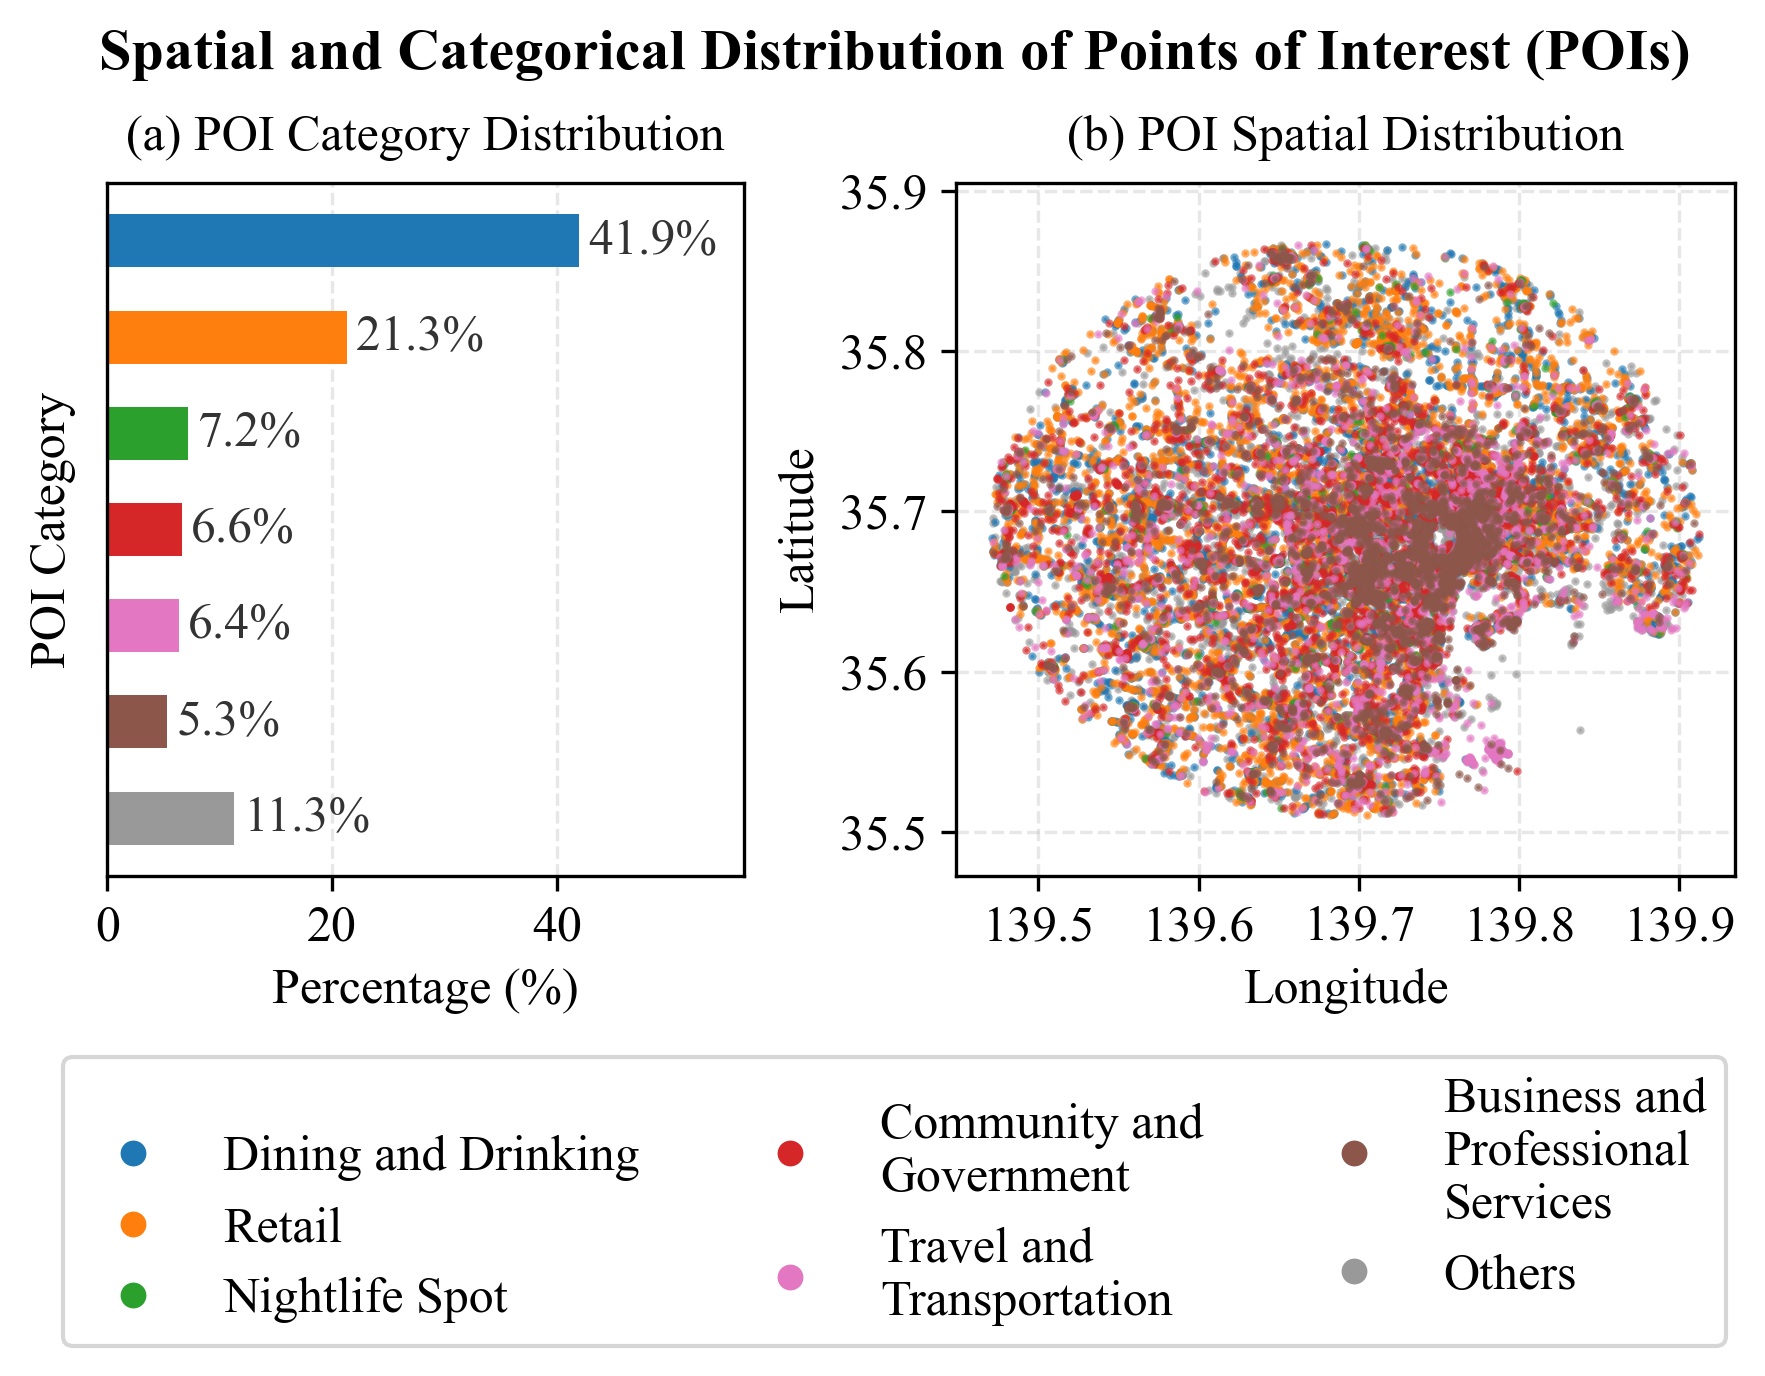
\includegraphics[width=\linewidth]{figure/poi_combined_analysis.png}
    \caption{Data Observation: (a) POI Category Distribution and (b) POI Spatial Distribution across the target region.}
    \label{fig:poi_dist}
\end{figure}

This ubiquitous presence of dining and retail facilities provides strong empirical justification for our methodological design. If absolute POI counts were evaluated directly, the overwhelming volume of restaurants would statistically mask the presence of critical but less frequent infrastructural POIs. Consequently, this severe imbalance necessitates the implementation of the TF-IDF preprocessing module discussed in Section~\ref{sec:method}, which effectively suppresses globally dominant categories to highlight the true functional signature of each spatial patch.


\begin{table}[htbp]
    \centering
    \caption{Statistical Summary of Users, POIs, and Spatial Grids}
    \label{tab:stats_summary}
    \setlength{\tabcolsep}{4pt}
    \begin{tabular}{lrrrr}
        \toprule
         & $n$ & Mean & Std. Dev. & Median \\
        \midrule
        \makecell[l]{Check-ins per User} & 2,293 & 250.20 & 221.57 & 173 \\
        \makecell[l]{Check-ins per POI} & 61,858 & 9.32 & 96.69 & 2 \\
        \makecell[l]{POIs per Grid (All)} & 19,158 & 3.10 & 5.22 & 1 \\
        \makecell[l]{POIs per Patch (Filtered)} & 1,233 & 18.98 & 10.49 & 15 \\
        \makecell[l]{Categories per Patch} & 1,233 & 4.58 & 1.40 & 4 \\
        \makecell[l]{Entropy per Patch} & 1,233 & 1.151 & 0.310 & 1.171 \\
        \bottomrule
    \end{tabular}
\end{table}
The spatial distribution reveals complex geographical clustering along main roads and transit stations, alongside large low-density areas in the western region. This highlights the need for a model capable of distinguishing between naturally dense hubs and structurally imbalanced aggregations. A statistical summary of the raw data and resulting spatial grids is provided in Table \ref{tab:stats_summary}.


\section{Experiments}
This section evaluates the effectiveness of the proposed framework through experimental setup, quantitative reconstruction analysis, qualitative analysis of TF-IDF preprocessing, FSCE topology, and latent-space behavior, followed by real-world case studies of POI additions.

\subsection{Experimental Setup}

\paragraph{Evaluation Protocol}
The dataset is split into an independent test set ($\text{test\_frac}=20\%$) which is completely excluded from any training or validation stages. The remaining data undergoes $k$-fold cross-validation with $N_{\text{splits}}=5$. Within each fold, we independently track four checkpoints corresponding to the epochs that achieve the lowest Mean Absolute Error (MAE), Mean Squared Error (MSE), Weighted Absolute Percentage Error (WAPE), and Poisson deviance on the validation set. During evaluation, the intact original data is used as the input. 

\paragraph{Evaluation Metrics}
All four metrics are first computed across the $C=10$ categories for a single patch, and then averaged over the entire batch of patches. Let $x_c$ be the ground truth category count and $\hat\lambda_c=\exp(\log\hat\lambda_c)$ be the Poisson rate parameter output by the decoder. We define $x_c\ln(x_c/\hat\lambda_c) = 0$ when $x_c=0$. We evaluate model performance using standard MAE and MSE, alongside WAPE and Poisson Deviance. WAPE is defined as the sum of absolute errors divided by the sum of true counts. Deviance is defined as $\frac{2}{C}\sum_{c=1}^{C}\left(x_c\ln(x_c/\hat\lambda_c)-(x_c-\hat\lambda_c)\right)$.

\paragraph{Baseline Models}
We select PCA, standard Autoencoder (AE), and Variational Autoencoder (VAE) as our primary baselines because they represent the core architectures suitable for mapping discrete count data into a continuous lower-dimensional latent space while performing reconstruction. PCA is configured with $n\_components=2$. The AE features a symmetric encoder-decoder architecture with 4 layers mapping to $d=2$. It shares the exact backbone of our proposed model but relies solely on a standard reconstruction objective.

\paragraph{Hyperparameters}
The network is trained using an Adam optimizer for $T=2000$ epochs with a mini-batch size of $B=256$ and a weight decay coefficient of $\gamma=1 \times 10^{-6}$. The learning rate follows cosine annealing, decaying from $\eta_{\max}=1 \times 10^{-2}$ to $\eta_{\min}=1 \times 10^{-3}$. For the denoising module, the thinning probability is set to $p=0.3$. For the graph construction and FSCE alignment, we configure the K-Means clusters to $K=8$ and the K-Nearest Neighbors to $k=10$. The UMAP kernel parameters are set to $a=1.0$ and $b=0.1$. During training, the FSCE edge mini-batch size is $B_e=256$, and the FSCE loss weight is gradually increased during a warm-up phase of $T_{\text{warmup}}=200$ epochs until it reaches $\lambda_{\max}=0.25$. The random seed is fixed at 0 across all experiments.


\subsection{Quantitative Analysis}

\paragraph{Reconstruction Performance}


This experiment validates that introducing topological constraints does not degrade the fundamental representation capability of the network. Table \ref{tab:main_results} compares our proposed architecture against standard baselines. The full model maintains reconstruction performance comparable to the best-performing DAE baseline while incorporating TF-IDF-based peer construction and FSCE topological regularization. This confirms that the proposed model successfully captures the underlying functional composition, providing a highly reliable foundation for calculating peer-relative contextual scores.


\begin{table}[h]
\centering
\caption{Main Reconstruction Performance Comparison}
\label{tab:main_results}
\begin{tabular}{p{4.5cm}ccc}
\toprule
Model & MAE & MSE & WAPE \\
\midrule
PCA & 0.7740 & 2.2116 & 0.4555 \\
AE & 0.6691 & 1.5303 & 0.3799 \\
VAE & 0.6906 & 1.5043 & 0.3941 \\
\midrule
Ours (DAE+FSCE+TFIDF) & \textbf{0.6487} & \textbf{1.3356} & \textbf{0.3720} \\
\bottomrule
\end{tabular}
\end{table}

\paragraph{Ablation Study}

To evaluate the contribution of each module, we systematically ablate the TF-IDF preprocessing, FSCE graph loss, and the Denoising mechanism. Table \ref{tab:ablation_results} groups the purely AE-based configurations and the DAE-based configurations. As shown in the table, the pure DAE model actually achieves the absolute best numerical scores in pure reconstruction metrics. Although the full model (DAE+FSCE+TFIDF) slightly trails behind the pure DAE in these specific numerical errors, this trade-off is entirely intentional. The addition of TF-IDF and FSCE imposes strict topological constraints that force the embeddings to reflect real-world functional relationships rather than optimizing solely for mathematical reconstruction. We explicitly detail how these added components crucially improve spatial separability and topological preservation in the subsequent qualitative analysis. Furthermore, the DAE-based models consistently outperform their AE counterparts, demonstrating that denoising is critical for stabilizing the latent space when these strong topological constraints are enforced.

\begin{table}[h]
\centering
\caption{Ablation Study on Reconstruction Performance}
\label{tab:ablation_results}
\begin{tabular}{p{4.5cm}ccc}
\toprule
Model & MAE & MSE & WAPE \\
\midrule
AE & 0.6691 & 1.5303 & 0.3799 \\
AE+FSCE & 0.6957 & 1.4584 & 0.3862 \\
AE+FSCE+TFIDF & 0.6725 & 1.6048 & 0.3770 \\
\midrule
DAE & \textbf{0.6442} & \textbf{1.3302} & \textbf{0.3651} \\
DAE+FSCE & 0.6503 & 1.3445 & 0.3685 \\
DAE+FSCE+TFIDF (Full) & 0.6487 & 1.3356 & 0.3720 \\
\bottomrule
\end{tabular}
\end{table}

\subsection{Qualitative Analysis}


\paragraph{Proving the Impact of TF-IDF Input}
To validate whether TF-IDF improves feature representation, we clustered patches using KMeans ($K=8$) before and after TF-IDF was applied. Figure \ref{fig:tfidf_impact} displays the resulting latent space distribution. Applying TF-IDF clearly mitigates the overwhelming influence of globally dominant categories, separating the data into distinct functional zones. This suggests that TF-IDF helps establish a more meaningful peer context in which similar areas can be compared during FSCE optimization.

\begin{figure}[h]
    \centering
    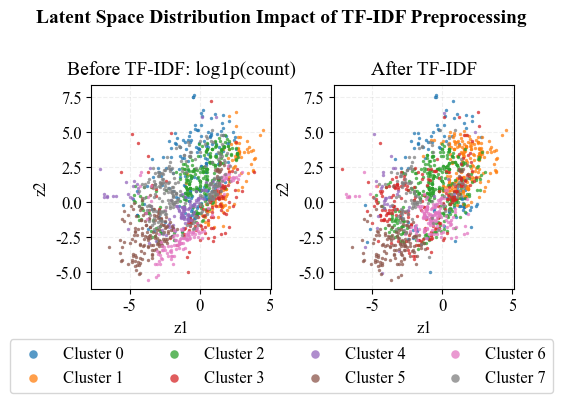
\includegraphics[width=\linewidth]{figure/latent.png}
    \caption{Latent Space Distribution Impact of TF-IDF Preprocessing. The right panel demonstrates improved cluster separability when TF-IDF suppresses overly common POI noise.}
    \label{fig:tfidf_impact}
\end{figure}



\paragraph{Proving the Helpfulness of FSCE}
We monitored the topological integrity during training by calculating the neighbor preservation rate, defined as the overlap of the top $k=10$ neighbors between the high-dimensional space and the 2D latent space. Figure \ref{fig:neighbor_preservation} confirms that the preservation rate reliably climbs as training progresses. This indicates that FSCE encourages the model to preserve functional neighbor relationships, so that patches close together in the latent space tend to share comparable functional compositions.
\begin{figure}[h]
    \centering
    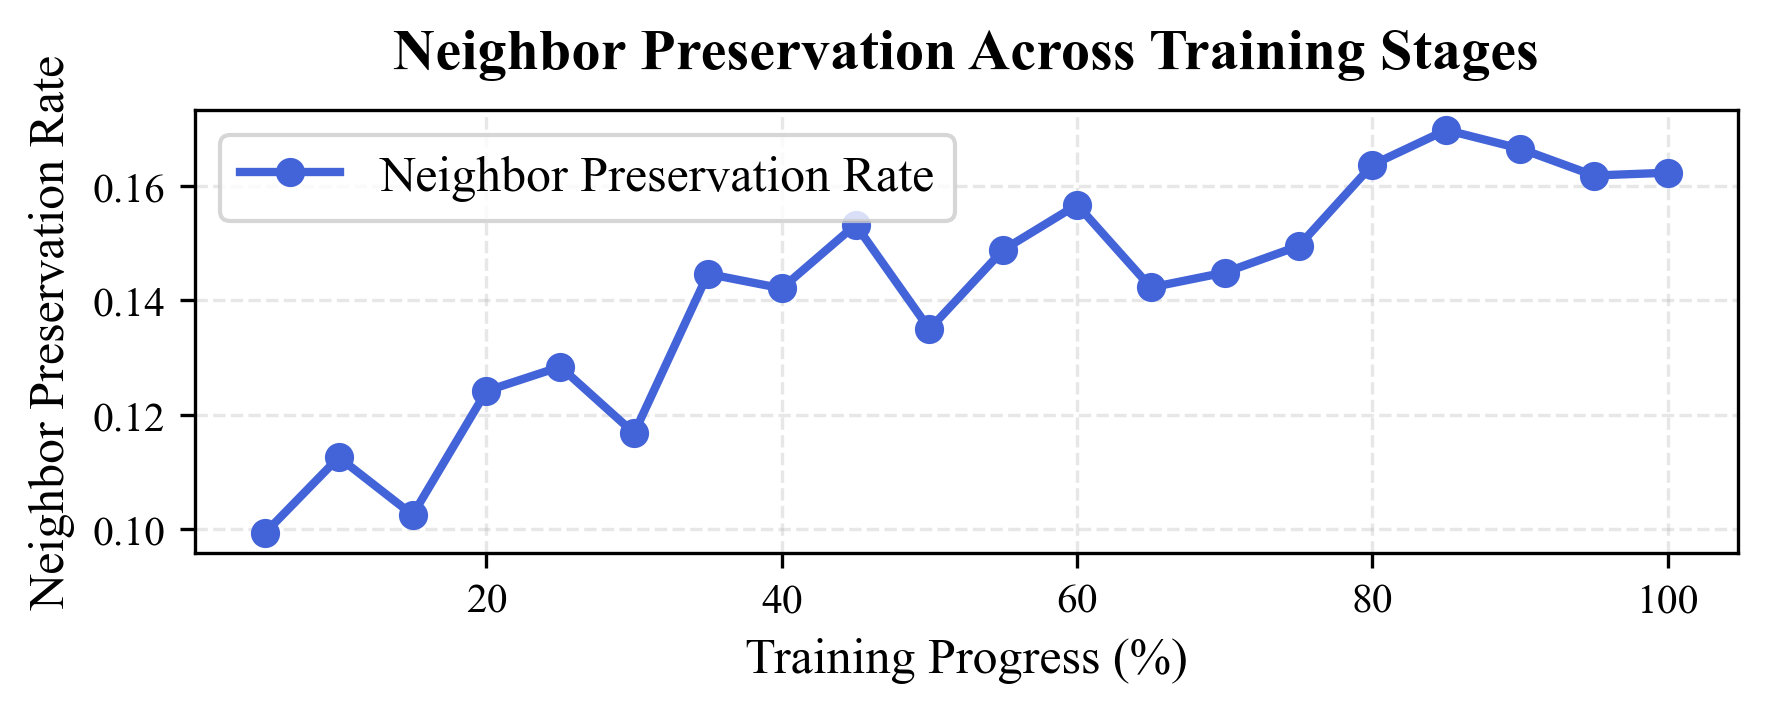
\includegraphics[width=\linewidth]{figure/neighbors.png}
    \caption{Neighbor Preservation across Training Stages. The steady increase indicates that FSCE anchors the low-dimensional embeddings to high-dimensional contextual realities.}
    \label{fig:neighbor_preservation}
\end{figure}



\paragraph{Observation of Latent Space Trajectory Shifts}
We visually analyzed the latent space offset caused by adding specific POI quantities to existing patches. Figure \ref{fig:latent_shift} maps these interventions across different model variants. While baseline models exhibit entangled shifts, our framework yields a smooth trajectory outward from the original patch locations. This visualization serves to illustrate how the latent state dynamically updates in response to new amenities, exposing the mechanical behavior of the structural assessment under the hood.


\begin{figure}[h]
    \centering
    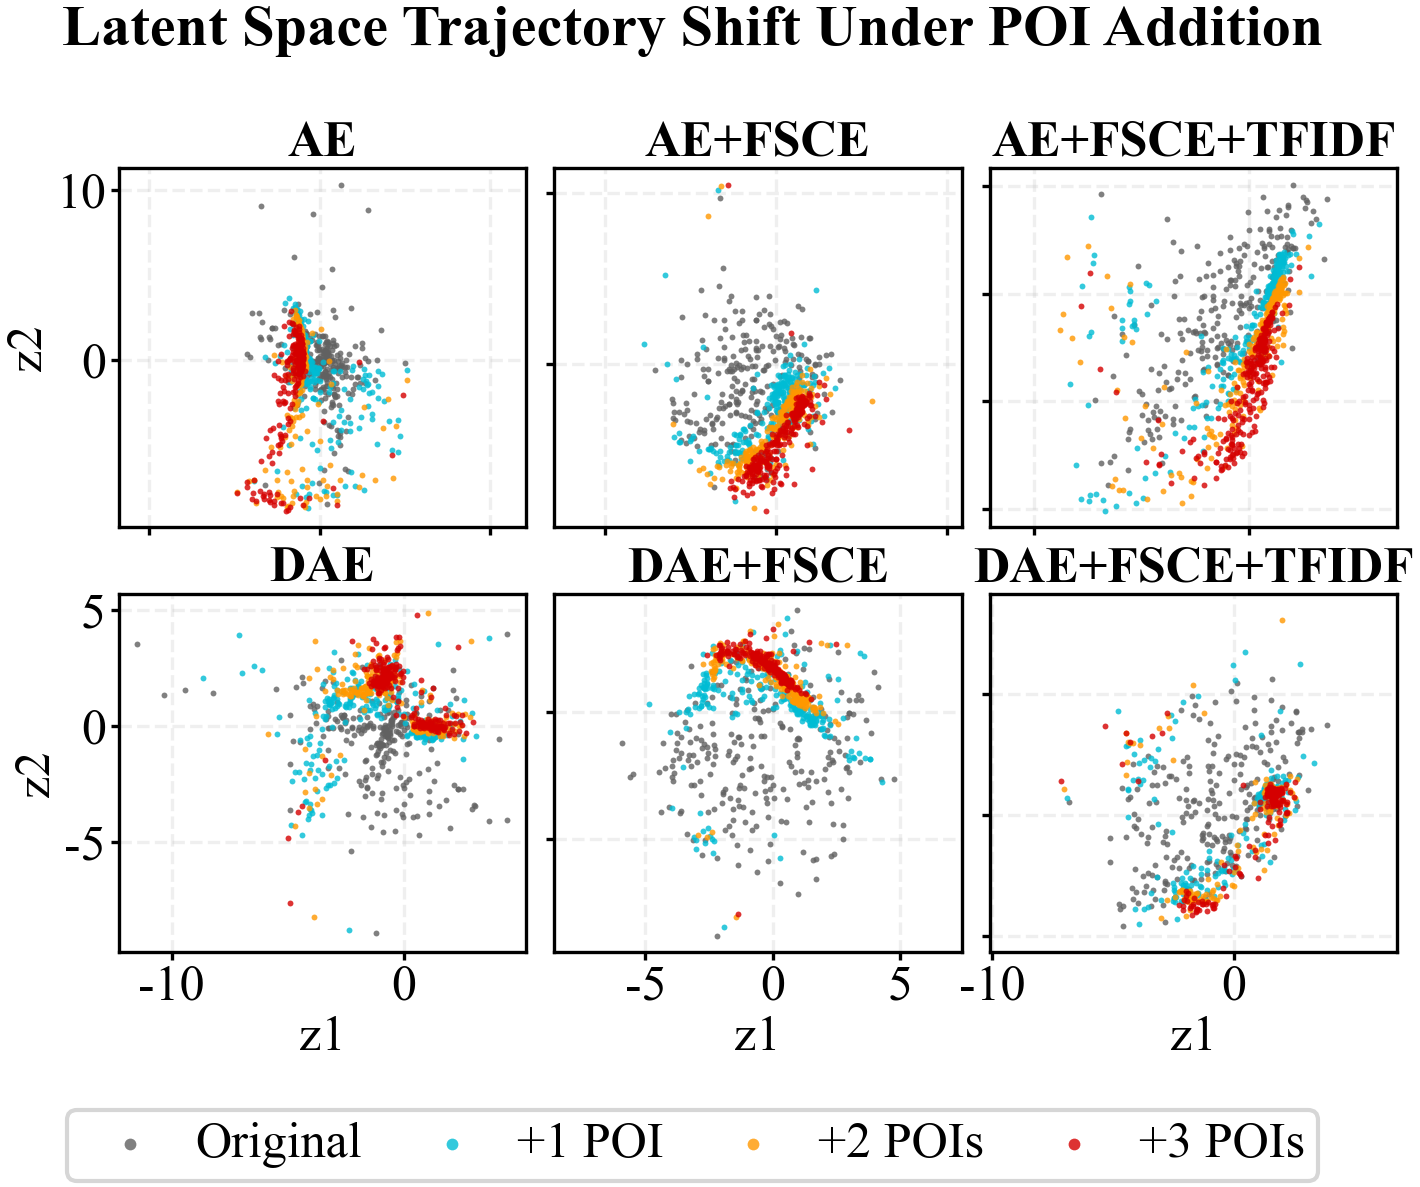
\includegraphics[width=\linewidth]{figure/latent_shift_all_steps.png}
    \caption{Latent Space Trajectory Shift: Tracking the movement of embeddings as 1, 2, or 3 POIs are injected into the input vector.}
    \label{fig:latent_shift}
\end{figure}


\subsection{Case Studies: Real-World Locational Evaluation}

\begin{figure}[h]
    \centering
    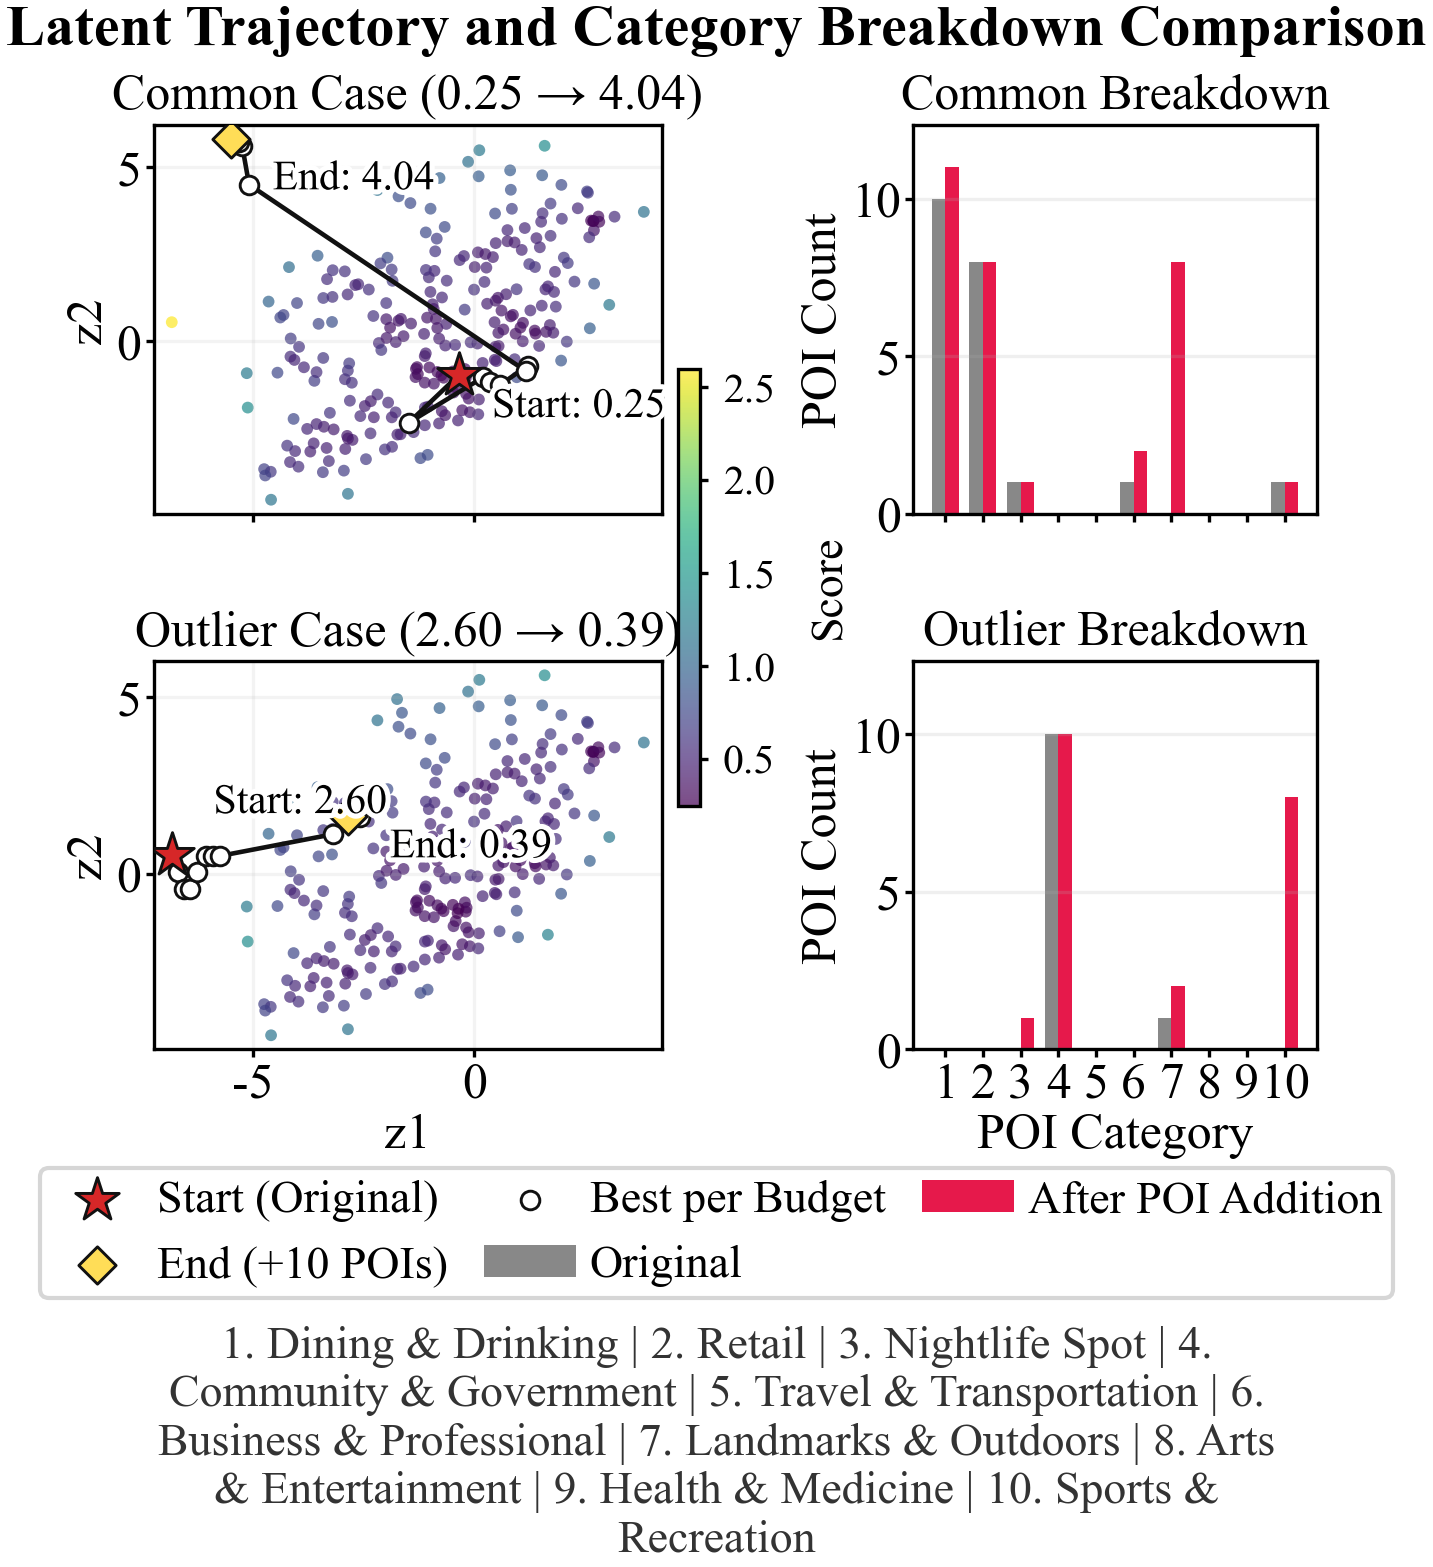
\includegraphics[width=\linewidth]{figure/image.png}
    \caption{Latent Trajectory and Category Breakdown Comparison. The top row shows a typical patch becoming an outlier due to over-concentration, while the bottom row shows an imbalanced patch achieving structural harmony through supportive POI additions.}
    \label{fig:case_study}
\end{figure}
To illustrate the behavior of the scoring mechanism, we selected real-world patches from the dataset and simulated POI additions using the budgeted search in Section~\ref{sec:method}. Since the additions are selected by optimizing the same score, these cases demonstrate how the score responds to interventions rather than independently validating planning effectiveness. 

Figure \ref{fig:case_study} illustrates both a common case and an outlier case. The outlier case represents a location initially lacking complementary infrastructure (starting score: 0.91). By systematically adding specific supportive POIs, the framework pulls this imbalanced patch back into a typical, functionally harmonious zone (ending score: 0.17). This illustrates how the score reflects the addition of complementary amenities that bring a patch closer to its functional peers. 

Conversely, the common case shows a standard, highly typical area (starting score: 0.08) receiving heavy POI additions. The framework identifies that these unchecked additions push the area outward into the latent periphery, transitioning it into a highly unique or potentially over-concentrated hub (ending score: 2.59). This illustrates the core premise of our study: rather than relying on absolute density caps, the score reflects whether a new POI addition keeps an area consistent with, or moves it away from, its functional context.


\section{Limitations and Future Work}
Although the proposed framework offers a peer-relative perspective on POI additions, several limitations remain. First, the score measures peer typicality, which we use as a proxy for structural balance; it has not yet been validated against independent evidence such as historical openings and closures, demand indicators, or expert assessment. Second, the Foursquare check-in data (2012--2013) are dated, subject to platform and demographic sampling biases, and reflect venues visited by users rather than a complete facility inventory. Because we focus on spatial composition, user and temporal information are excluded, so the model does not observe actual demand, capacity, accessibility, or commercial viability. We envision the system as an exploratory screening tool for urban planners and local communities in the early stage of facility planning, where candidate additions can be compared before detailed feasibility studies. Future work will validate the score with recent POI data, observed facility changes, and planner feedback.

\section{Conclusion}

This study introduced a peer-relative spatial decision support system designed to evaluate urban structural balance and assess the suitability of new POI additions. By integrating TF-IDF preprocessing with a Denoising Autoencoder and FSCE topological constraints, our framework shifts locational evaluation from absolute density estimation toward a peer-relative contextual assessment. Experimental findings suggest that TF-IDF suppresses globally dominant categories to clarify functional boundaries, while the joint optimization strategy helps anchor low-dimensional representations to the functional peer structure. The case studies further illustrate how the system characterizes whether new facilities move an area toward or away from its functional peers.

\begin{acks}
This work was supported in part by the National Science and Technology Council of Taiwan, R.O.C., under Contracts 114-2121-M-005-006, and 115-2121-M-005-005. The authors also used Claude and Gemini to polish the grammar and language of this manuscript. The authors reviewed all content and take full responsibility for the content of this publication.
\end{acks}
%
%% The next two lines define the bibliography style to be used, and
%% the bibliography file.
\bibliographystyle{ACM-Reference-Format}
\bibliography{sample-base}

\end{document}
\endinput
%%
%% End of file `sample-sigconf.tex'.
